
\documentclass{article}
\usepackage{tikz}

\begin{document}
    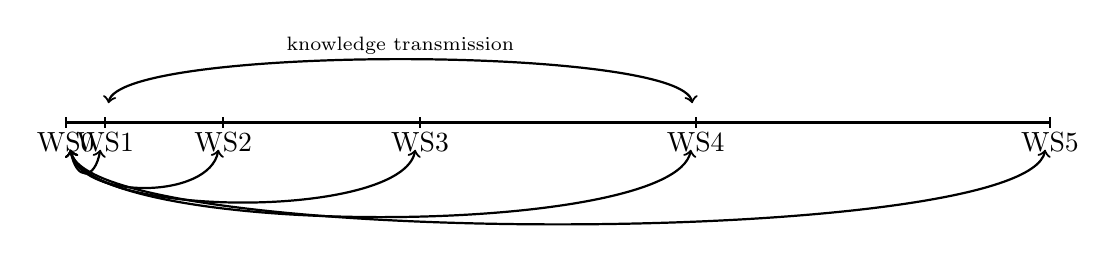
\begin{tikzpicture}[thick,scale=.5]
	\coordinate (WS0) at (0,0);
	\coordinate (WS1) at (1,0);
	\coordinate (WS2) at (4,0);
	\coordinate (WS3) at (9,0);
	\coordinate (WS4) at (16,0);
	\coordinate (WS5) at (25,0);
	\draw[thick,-] (0,0) -- (25,0) node[anchor=north west] {};   
	\foreach \x in {0,1,4,9,16,25}
		\draw (\x cm,4pt) -- (\x cm,-4pt) node[anchor=north] {};
	\draw (WS0) node[anchor=north]{WS0};
	\draw (WS1)node[anchor=north]{WS1};
	\draw (WS2)node[anchor=north]{WS2};
	\draw (WS3)node[anchor=north]{WS3};
	\draw (WS4)node[anchor=north]{WS4};
	\draw (WS5)node[anchor=north]{WS5};

	\draw [black,shorten <= 0.25cm, shorten >= 0.25cm, <->] (WS1) to[out=80,in=100,distance=2cm] node[above,font=\scriptsize]{knowledge transmission} (WS4); 
	\draw [black,shorten <= .35cm, shorten >= .35cm, <->] (WS0) to[out=-80,in=-100,distance=1.5cm	]  (WS1);
	\draw [black,shorten <= .35cm, shorten >= .35cm, <->] (WS0) to[out=-80,in=-100,distance=2cm	]  (WS2);
	\draw [black,shorten <= .35cm, shorten >= .35cm, <->] (WS0) to[out=-80,in=-100,distance=2.5cm	]  (WS3);
	\draw [black,shorten <= .35cm, shorten >= .35cm, <->] (WS0) to[out=-80,in=-100,distance=3cm	]  (WS4);
	\draw [black,shorten <= .35cm, shorten >= .35cm, <->] (WS0) to[out=-80,in=-100,distance=3.25cm	]  (WS5);
    \end{tikzpicture}
\end{document}

